\documentclass{standalone}
\usepackage{tikz}

\begin{document}
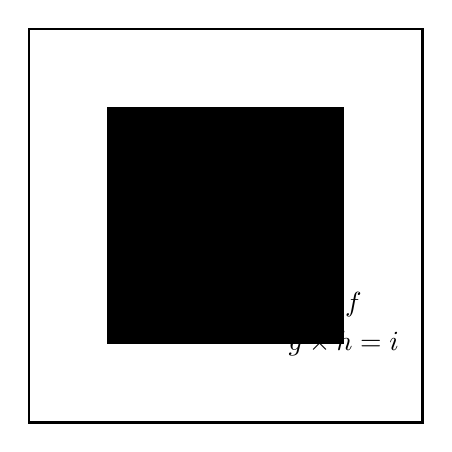
\begin{tikzpicture}[scale=0.5]
    % Draw the outer white square with a black border
    \draw[fill=white] (0,0) rectangle (10,10);
    \draw[black, thick] (0,0) rectangle (10,10);

    % Draw the inner black box with mathematical symbols and equations
    \draw[fill=black] (2,2) rectangle (8,8);
    
    % Add some mathematical symbols and equations inside the black box
    \node at (5,5) {$x^2 + y^2 = z^2$};
    \node at (6,4) {$a + b = c$};
    \node at (7,3) {$d - e = f$};
    \node at (8,2) {$g \times h = i$};
\end{tikzpicture}
\end{document}